\chapter{Evaluating dark matter signals}
The main goal of the thesis is to investigate if certain dark matter signals can be detected after the high luminosity upgrade. One immediate worry is that the background will be large in comparison to the signal, thus making it undetectable. 

The following signals models have been used:
\textbf{Here only the operators should be explained, or different models. The names and the MC here or in appendix?} They are explained somewhat in the introduction.
Each of these has been evaluated in different signal regions and the detectability has been evaluated using a statistical P-value. This process has been performed at different pile-up values. 

\textbf{What background existed? How was it simulated in MC? Should that be here or in appendix?}


Dont mention, but good to know. Used METpt in all histograms, with the weight as in main.C and mainclass.C. 


\section{Signal to background ratio}
What I am doing now, looking at what signal? What are the different background processes? What and why was the weight used?

Signals should be explained somewhat in the introduction.



Look at presentation, is it worth bringing up the first signal regions when the data has already been filtered? Should that be here?
 
\subsection{Selection criteria}
What criteria were used and more importantly why? It is quite important that you can explain why this was used.

For different purposes different selection criteria or regions are used. These are a set of criteria specified to enhance the area of interest. For instance, if simulating a specific signal one wants to find as many ways as possible to diminish the background. This so that when searching experimentally, the signal will be easier to detect.

These can be quite general cuts, there are only some things to take into consideration. 
\begin{itemize}
\item If experimental, what limitations are set by the detectors? Are there some criteria already?
\item If simulated, is there some criteria set in the generator?
\item Are there criteria which must be set since there is to much uncertainty in the data? or a large effect of pile up?
\end{itemize}


\subsection{Verifying background data} 	
To verify that the background data was correct it was compared with \citep{ATLAS-CONF-2012-147}, in which the luminosity if 10 fb$^{-1}$ and thus the expected values from the paper scaled up with a factor 100. \textbf{Also, somewhat unexpectedly is that the difference in center of mass energy required the cross-sections to be much lowered than compared with the upgrade.} The signal region used in the article were the following:
\begin{table}[h]
\begin{center}
\begin{tabular}{l}
\hline
Selection Criteria \\ \hline
Jet veto, require no more than 2 jets with $p_T > 30 GeV$ and $|\eta| < 4.5$ \\
Lepton veto, no electron or muon \\
Leading jet with $|\eta| < 2.0$ and $\Delta \phi (jet, E_T^{Miss})>0.5$ (second-leading jet) \\ \hline
\end{tabular}
\begin{tabular}{l l l l l l}
signal region & SR3p & SR4p \\ \hline
minimum leading jet p$_T$ (GeV) & 350 & 500 \\
minimum E$^{Miss}_T$ (GeV) & 350 & 500 \\ \hline
\end{tabular}
\label{tab:oldsr}
\caption{The signal regions}
\end{center}
\end{table}






The article has several different signal regions, the difference is the last item, unfortunately since the simulated events are already filtered before the analysis only one of the regions could be used.

NEW WITH 350 as SR3 and 500 as SR4 and expected (Scaled to 1000 fb$^{-1}$) thus scaled a factor 100.
\begin{table}[ht]
\begin{center}
\begin{tabular}{|l|l|l|l|l|}
\hline
Process & SR3p & Expected SR3p & SR4p  & Expected SR4p \\ \hline
Z$\rightarrow\nu\nu$&140298&152000&25250.3&27000 \\
W$\rightarrow\tau\nu$&40700.8&37000&5861.74&3900 \\
W$\rightarrow e\nu$&11229&11200&1506.58&1600 \\
W$\rightarrow\mu\nu$&13727.1&15800&1872.32&4200 \\ \hline
Total background&205955&218000&34491&36700 \\ \hline
\end{tabular}
\caption{Comparison of the simulated and expected events from \citep{ATLAS-CONF-2012-147}.}
\label{tab:Compare1}
\end{center}
\end{table}

The scaling is done by multiplying by a factor 100.
In \tableref{tab:Compare1} a comparison has been made. It can be seen that the simulated events and expected events coincide on all accounts apart from W$\rightarrow\tau\nu$, W$\rightarrow\mu\nu$ and thus the total as well. \textbf{This can be explained by better separation of $\mu$,$\tau$ and missing energy.} 
Tau can not be reconstructed as jets in the code, they can in reality!

\subsection{Figures of merit}
\textbf{P-value, info from Majas phd thesis. Is there a source? Should there be a figure?}

To be able to evaluate different signal regions and different signal models, a figure of merit p is used. The value p is the probability for an assumed hypothesis to be correct, thus a good signal region will yield a low value. The assumed hypothesis is that the background and its fluctuations is measured over the signal plus background.

Assuming the expected number of background events are B $\pm \sigma_B$ where $\sigma_B$ is the quadratic sum of the statistical error from Monte Carlo, the statistical error from the control region and the systematic errors. The expected number of signals is S, assumed without fluctuation. 

If no uncertainty in B or S is assumed, then the number of expected events, N, in the signal region should follow a Poisson distribution as such:
\begin{equation}
\text{P(N|S+B)}=\frac{e^{-(S+B)}(S+B)^N}{N!}
\end{equation} 

However since there is an uncertainty in the background, the probability distribution P(N|S+B) must be convoluted with a Gaussian function:
\begin{equation}
 \text{G(N$_B$|B,$\sigma_B$)}=\frac{1}{\sigma_B \sqrt{2 \pi}} e^{-\frac{(N_B-B)^2}{2\sigma_B^2}}
\end{equation}
where N$_B$ is the expected number of background events. The convolution is done using N$_B$ as N resulting in the total probability density function:
\begin{align}
\text{F(N|S+B},\sigma_B) &= \text{P(N|S+N$_B$)$\ast$G(N$_B$|B,$\sigma_B$)}= \notag \\
&=\int\limits_{-\infty}^{\infty}P(N|N_B - (S+B))G(N_B|B,\sigma_B) dN_B
\end{align}
This leads to the probability of the signal plus background fluctuation to B events being obtained by summing the probability function from N=0 to N=B.
\begin{equation}
p = \sum\limits_{i=0}^{B} \int\limits_{-\infty}^{\infty} \text{P(i|N$_B - $(S+B))G(N$_B$|B,$\sigma_B$)} dN_B
\end{equation}



\subsection{D5 operators}
Discuss M*, and the difference in mDM. From presentation given, 3-4 April. 

As described in the introduction \textbf{reference?}, one of the signals is modelled using the D5 operator. In this thesis two different scenearios were used, one at a dark matter mass of 50 GeV and one at 400 GeV.

\subsection{Light vector mediator models}
Discuss Mm, width, and the difference in mDM. From presentation given, 3-4 April.

As described in the introduction \textbf{reference?}, the other signal model is a vector mediator model. The data available is: two different widths M/3 and M/8pi. \textbf{M?!?}
two different mDM, 50 GeV and 400 GeV and finally a variety of mediator masses. 

\subsection{Susy models?}
\section{Other selection criteria and observables}
New signal regions.
\begin{table}[h]
\begin{center}
\begin{tabular}{l}
\hline
Selection Criteria \\ \hline
Jet veto, require no more than 2 jets with $p_T > 30 GeV$ and $|\eta| < 4.5$ \\
Lepton veto, no electron or muon \\
Leading jet with $|\eta| < 2.0$ and $\Delta \phi (jet, E_T^{Miss})>0.5$ (second-leading jet) \\ \hline
\end{tabular}
\begin{tabular}{l l l l l l}
signal region & SR0 & SR1 & SR2 & SR3 & SR4 \\ \hline
minimum leading jet p$_T$ (GeV) & 120 & 350 & 600 & 800 & 1000 \\
minimum E$^{Miss}_T$ (GeV) & 120 & 350 & 600 & 800 & 1000 \\ \hline
signal region & SR0 & SRa & SRb & SRc & SRd \\ \hline
minimum leading jet p$_T$ (GeV) & 350 & 350 & 350 & 350 & 350 \\
minimum E$^{Miss}_T$ (GeV) & 120 & 350 & 600 & 800 & 1000 \\ \hline
\end{tabular}
\label{tab:newsr}
\caption{The new signal regions}
\end{center}
\end{table}

\section{Mitigating the effect of the high luminosity}
Something pile-up
Something as seen in validation of... the effect is quite minute for high energy values and does not at all affect leptons or photons. Mention that the effect is on a trigger level, that the lowest SR will be lost.

Even though this was envisioned as the primary focus of the thesis, it was shown that the effect of pile-up is minute for these high signal regions. Thus the focus was shifted to perform a more in-depth mono-jet analysis of different DM signal models.
\section{Results}
\subsection{Limit on M*}
The mass suppression scale.
Give at 1000fb-1. And for the different signal regions.
\textbf{ASK CHRISTOPHE FOR A GOOD EXPLANAITION OF M* and why there can be limits!}

For the new signal regions: \textbf{Include a table of the limits for truth and Reco.}
 \begin{figure}[H] %!ht
    \subfloat[ \label{fig:SRnewM:1}]{%
     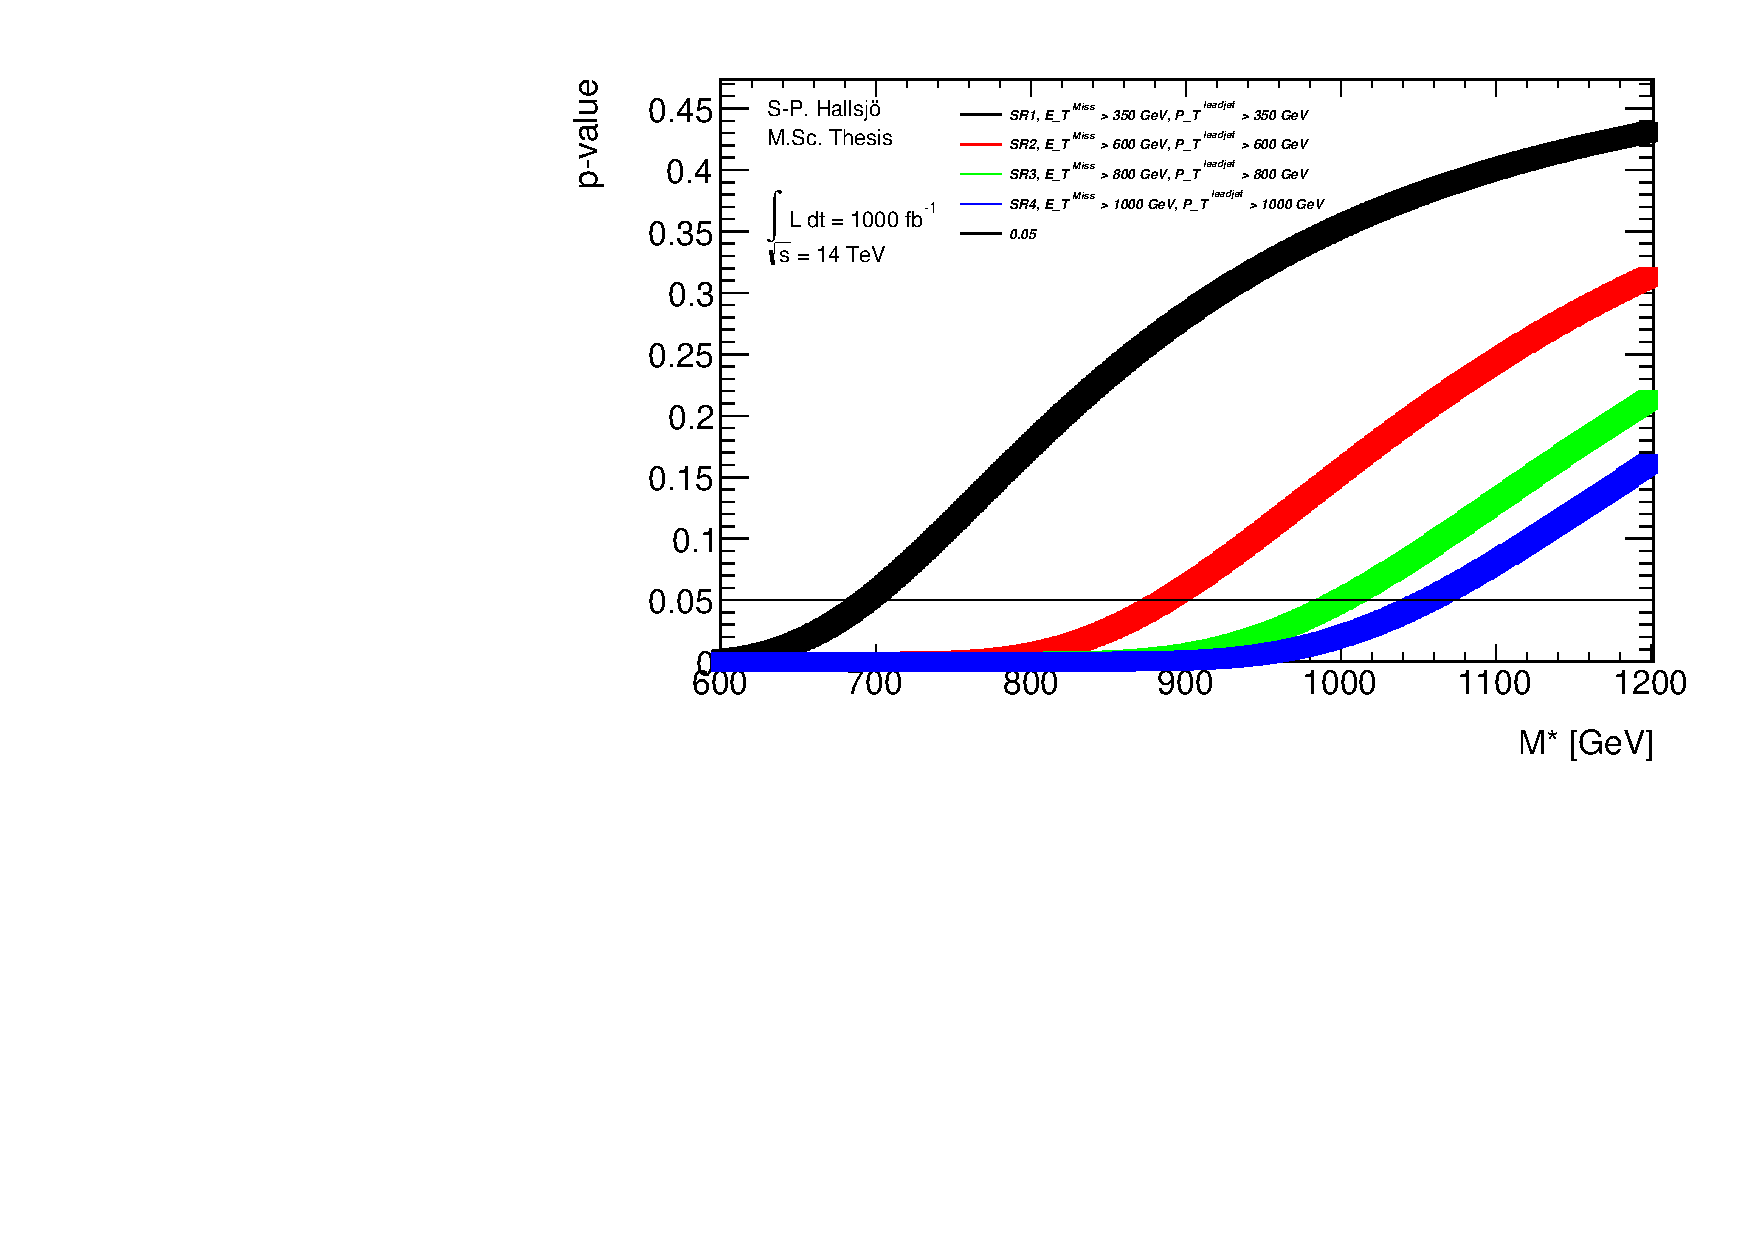
\includegraphics[width=0.5\textwidth]{pvaluemm.pdf}
    }
    \hfill
    \subfloat[ \label{fig:SRnewM:2}]{%
      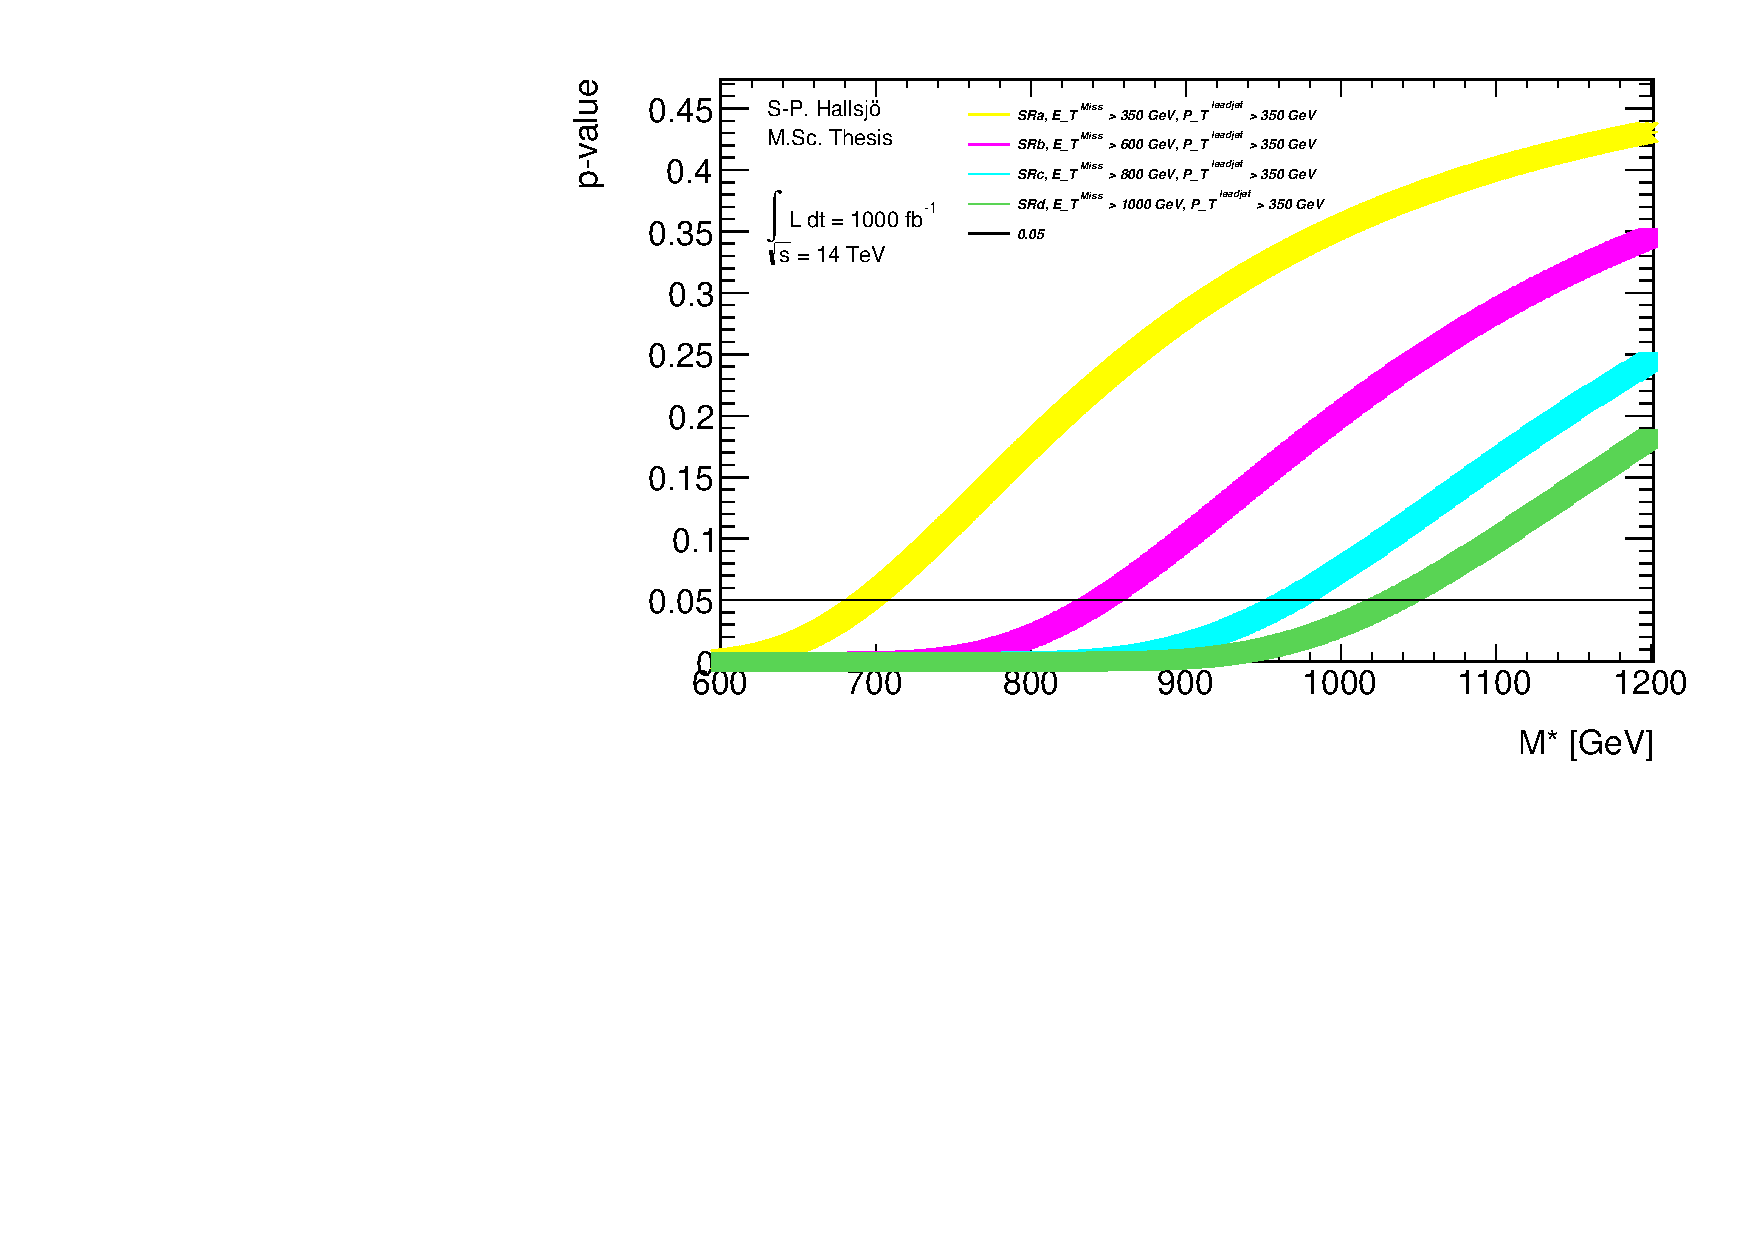
\includegraphics[width=0.5\textwidth]{pvaluemm2.pdf}
    }
    \caption{On a truth level.}
    \label{fig:SRnewM}
  \end{figure}

\subsection{Effect of pile-up on M*}
Hardly any effect. 10 \% or in that vicinity.

\subsection{Previous results}
Valerios paper for instance.
Preliminary not that much better results for 1000fb-1 and 14TeV.

The whole discussion with Steven and David.
\subsection{Limit on mediator mass}
Are there previous results?
Signal vs background plot in normal and log scale for one of the vector mediator models, to be able to evaluate all the different models the so called p-value was used in different signal regions. Below are two figures showing one of the vector mediator models in SR3.
 \begin{figure}[H] %!ht
    \subfloat[Signal on background plot for E$^{Miss}_T$ on reco level in SR3. \label{fig:sigback:1}]{%
     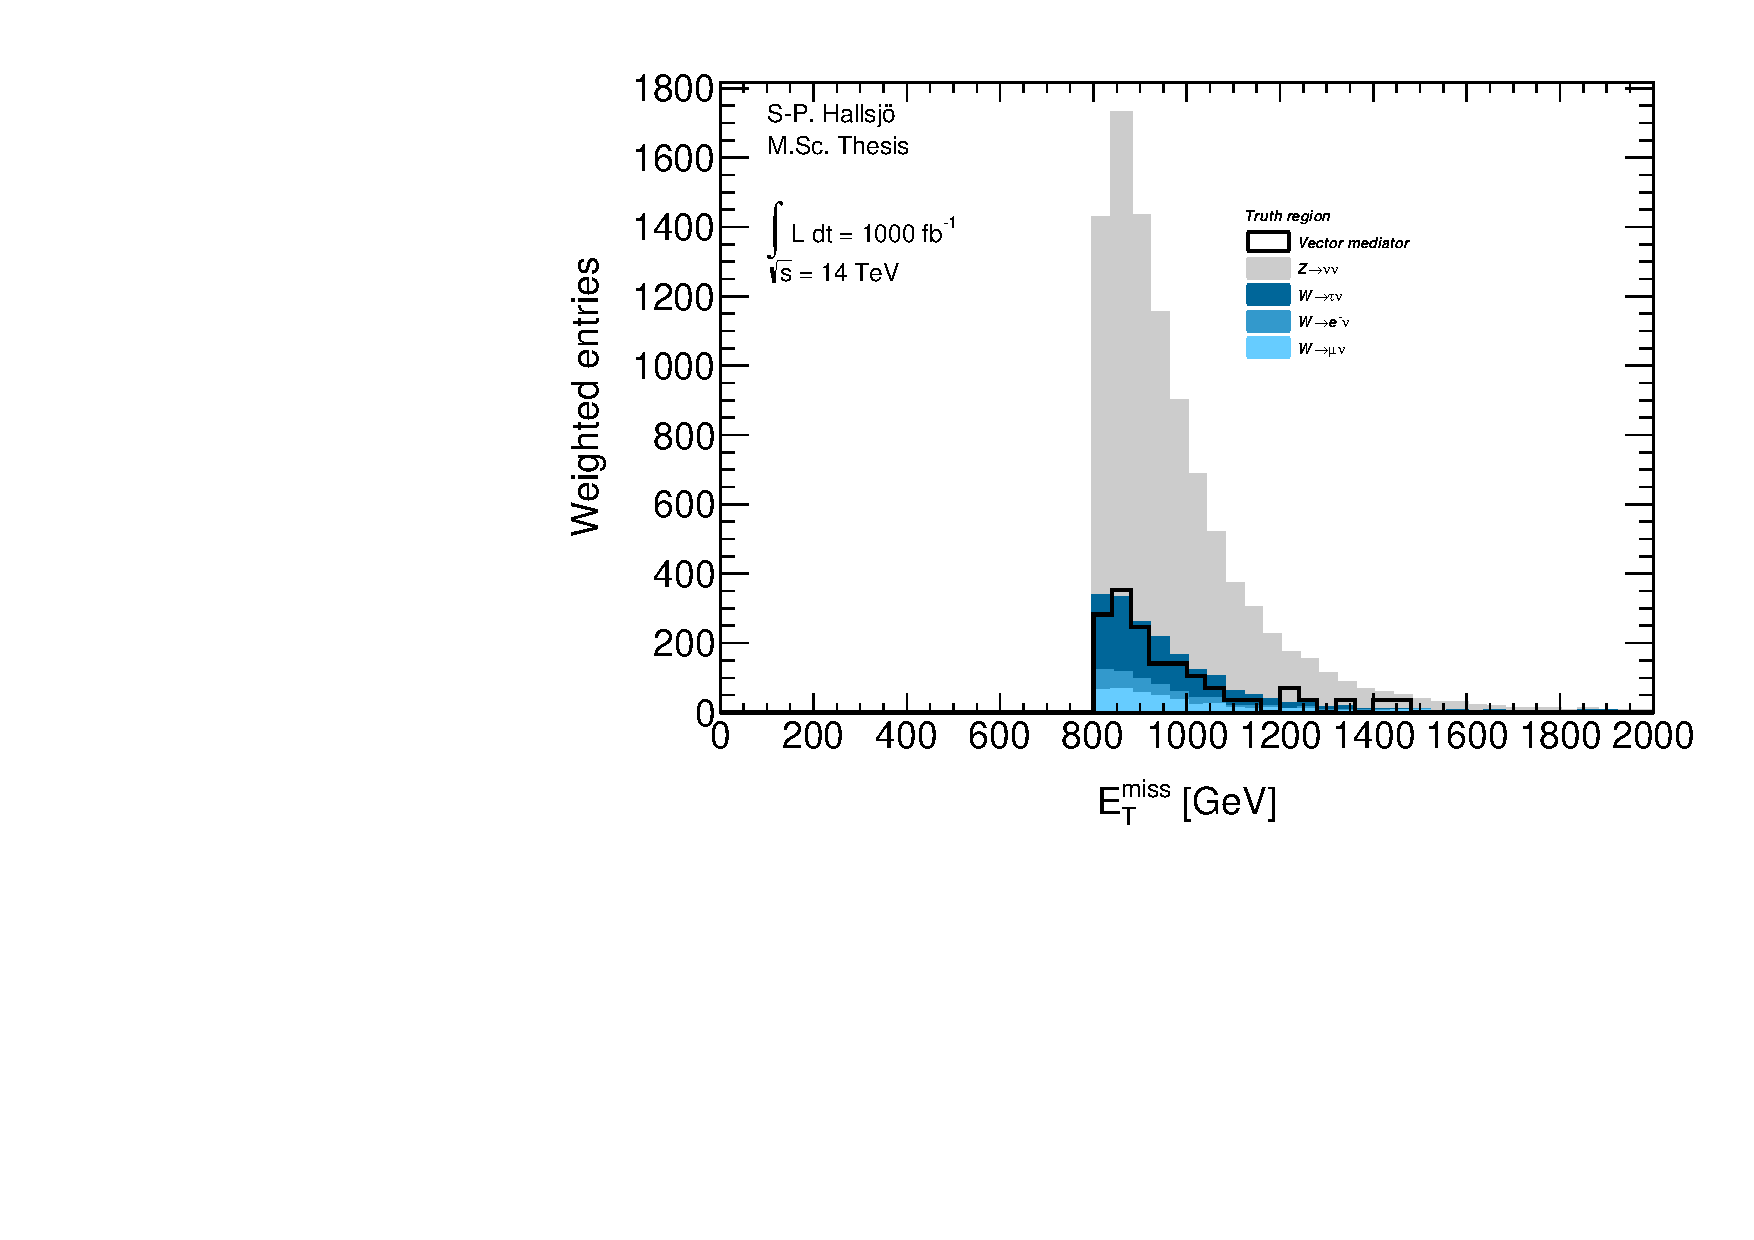
\includegraphics[width=0.5\textwidth]{exsig2sr3.pdf}
    }
    \hfill
    \subfloat[The same as a) with log scale on the y-axis \label{fig:sigbacktau:2}]{%
      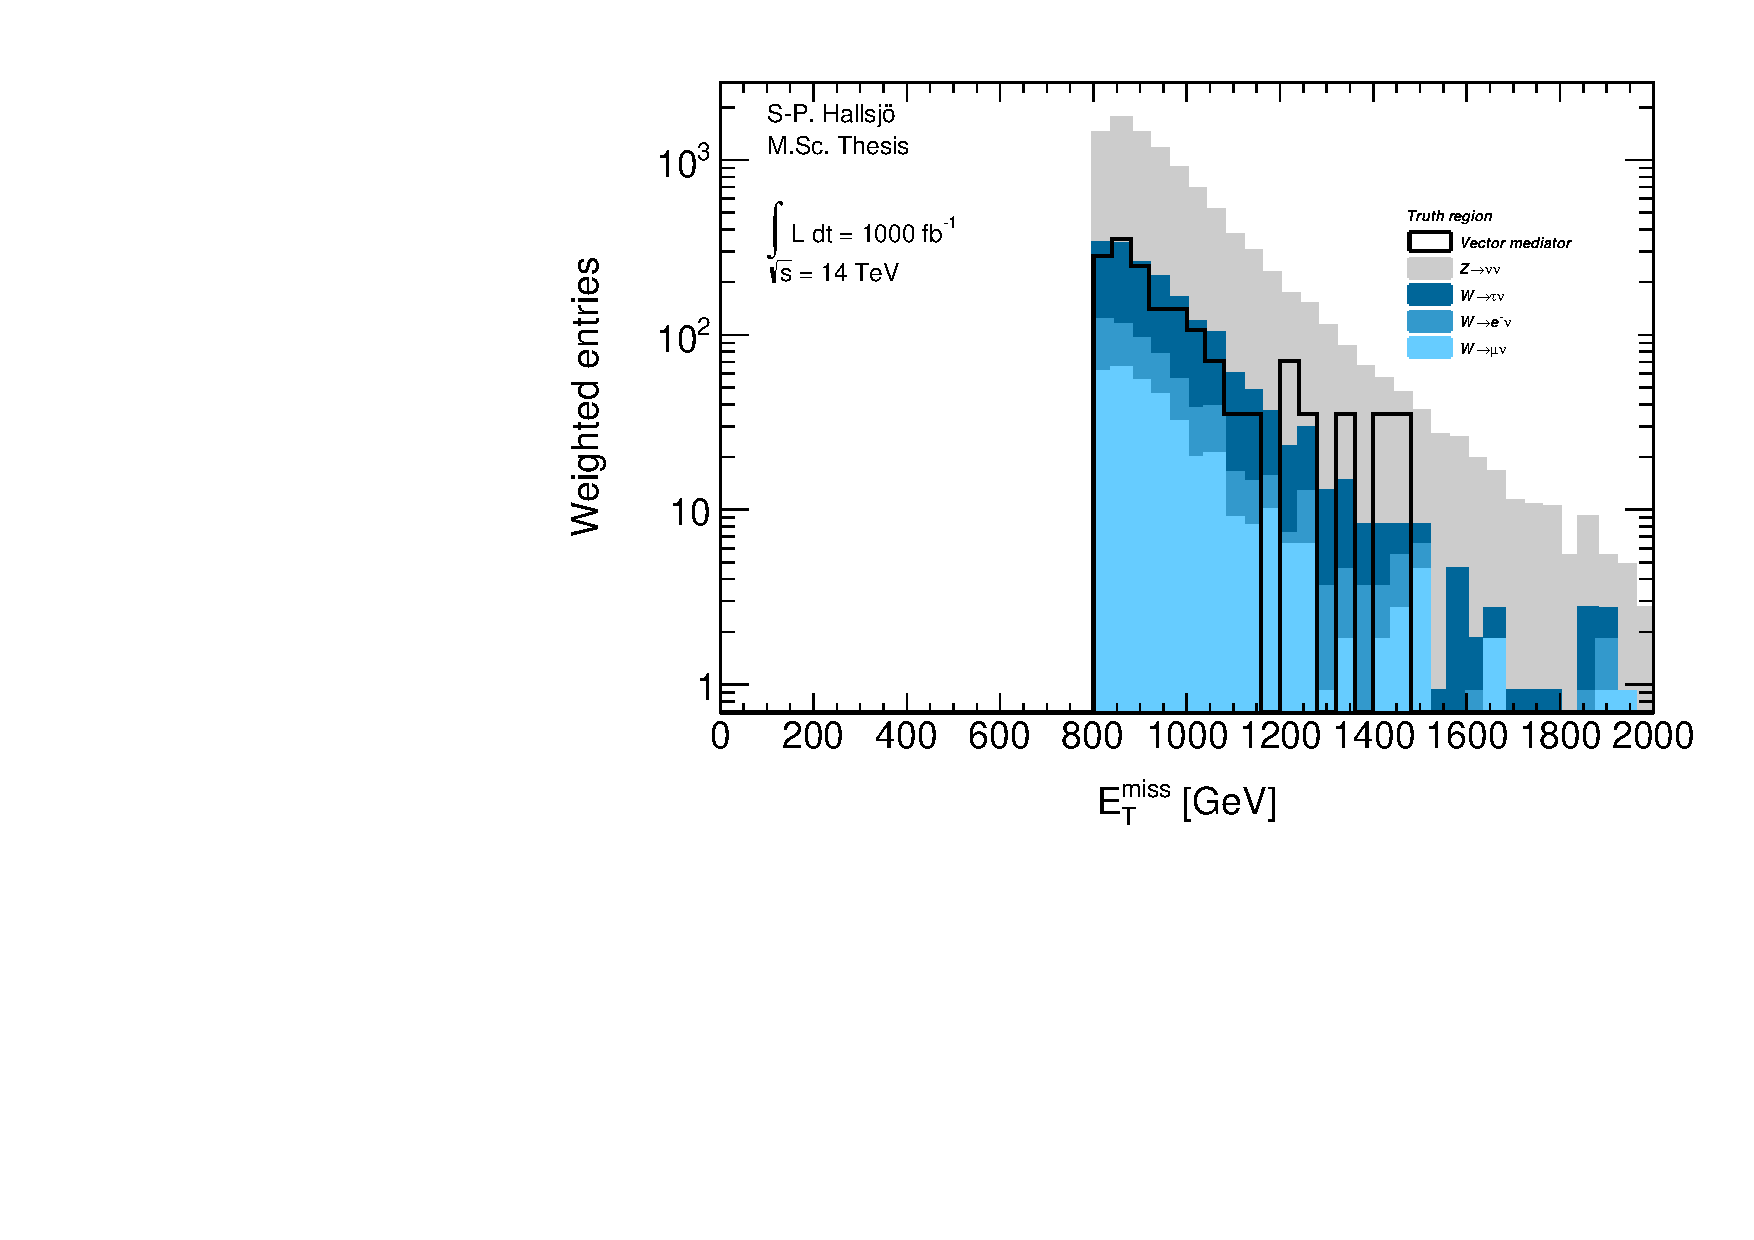
\includegraphics[width=0.5\textwidth]{exsig2sr3log.pdf}
    }
    \caption{Signal on background plot to illustrate the a general plot. }
    \label{fig:sigback}
  \end{figure}

To set a limit on the mediator mass the p-value was calculated in different signal regions for the different signal models with different mediator mass. This resulted in the following plot:


\subsection{Effect of pile-up on mediator mass}
Check the different cases for reco and truth to see what happens.
\section{Discussion}
\section{Conclusion}